\documentclass[a4paper,12pt]{book}
\usepackage[utf8]{inputenc}
\title{}
\author{Rachel Morris}
\date{\today}

\usepackage{rachwidgets}
\usepackage{fancyhdr}
\usepackage{lastpage}
\usepackage{dirtree}
\usepackage{boxedminipage}

\newcommand{\laChapter}{5.3\ }

\pagestyle{fancy}
\fancyhf{}
\lhead{CS 211}
\chead{Fall 2017}
\rhead{Ch \laChapter Exercise}
\rfoot{\thepage\ of \pageref{LastPage}}
\lfoot{\scriptsize By Rachel Morris, last updated \today}

\renewcommand{\headrulewidth}{2pt}
\renewcommand{\footrulewidth}{1pt}

\begin{document}

    %\toggletrue{answerkey}
    \togglefalse{answerkey}
    
    %------------------------------------------------------------------%
    %- Exercise Begin -------------------------------------------------%
    %------------------------------------------------------------------%

    %------------------------------------------------------------------%
    \section*{1. Review}

        \begin{intro}{CS 210 - Functions} ~\\
            $f : A \to B$ specifies a function named $f$,
            with some set of inputs ($A$, the domain), and a set of
            outputs ($B$, the codomain). The function $f$ associates
            each input $A$ with one and only one output from $B$.

            \begin{center}
                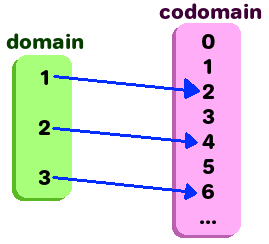
\includegraphics[height=4cm]{images/5-3-function.png}
            \end{center}
                
            A function $f$ with domain $\{1, 2, 3\}$,
            a codomain $\mathbb{N}$, and the rule, $2k$.
        \end{intro}

        % - QUESTION --------------------------------------------------%
        \begin{question}{1}{5\%}
            Let $f$ be the function with the domain $\{a, b, c\}$ and codomain
            $\{1, 2, 3\}$ defined by the set of ordered pairs:
            $\{(a, 2), (b, 3), (c, 1)\}$. Complete the arrow diagram.

            \begin{center}
                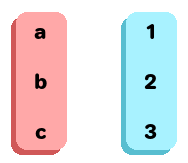
\includegraphics{images/5-3-question-function.png}
            \end{center}
        \end{question}

        \newpage
        \begin{intro}{CS 210 - Binary Relations} ~\\
            A binary relation $R$ has
            a domain $A$, a codomain $B$, and its rule is the subset of
            $A \times B$ (the Cartesian* product of $A$ and $B$).

            \begin{center}
                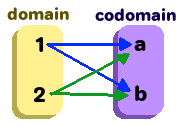
\includegraphics[height=3.5cm]{images/5-3-relation.png}                
            \end{center}

            \begin{center}
                Domain: $A = \{1, 2\}$, Codomain: $B = \{2, 3\}$, ~\\
                Rule: $L = \{(1, 2), (1, 3), (2, 2), (2, 3)\}$.
            \end{center}

            \paragraph{Cartesian product:}
            a Cartesian product is a mathematical operation that returns a set (...) from multiple sets.
            That is, for sets $A$ and $B$, the Cartesian product $A \times B$ is the set of all ordered pairs
            $(a, b)$ where $a \in A$ and $b \in B$.
            \footnote{From https://en.wikipedia.org/wiki/Cartesian\_product}
            \\
            So if we took the Cartesian product from $A$ and $B$ above,
            the result would be $L$.
        \end{intro}

        % - QUESTION --------------------------------------------------%
        \begin{question}{2}{6\%}
            Finish the diagram for the relation $R_{1}$ on the set $\{1, 2, 3, 4\}$ with the rule
            $(x, y) \in R_{1}$ if $x \leq y$
            
            \begin{wrapfigure}{r}{0.25\textwidth}
                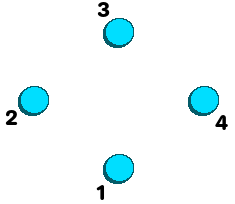
\includegraphics[height=4cm]{images/5-3-question-relation.png}
            \end{wrapfigure}

            \paragraph{Hints:}
            \begin{itemize}
                \item If a relationship exists between some point ($x$, $y$),
                    it means that the value of $x$ is $\leq$ $y$. This will
                    be represented graphically as an arrow starting at $x$ and
                    pointing to $y$.
                \item For node (1), it is \textit{less than} (2), (3), and (4),
                    and it is equal to (1), so it will have arrows pointing
                    to all of these.

                \item For node (4), it is only $\leq$ itself, so it will only
                    have an arrow looping back to itself.
            \end{itemize}
        \end{question}
        
    \newpage
    %------------------------------------------------------------------%
    \section*{2. Subsets}

        \begin{intro}{Permutations:}
            A \textbf{permutation} is an ordered list where elements cannot repeat.
            For example, if we have a set of numbers \{1, 2, 3\}, then
            we could have permutations (1, 2, 3), (1, 3, 2), (2, 1, 3), (2, 3, 1),
            and so on. ~\\

            Permutations of length $r$, pulling elements from
            $\{1, 2, ..., n\}$, can be written as $P(n,r)$. ~\\

            $P(n, n)$ can be calculated as $n!$ ($n$-factorial). If we are
            not selecting all items from $\{1, 2, ..., n\}$, then we can
            compute the amount of results as         
<<<<<<< HEAD
            $P(n, r) = \frac{n!}{(n-r)!}$.
=======
            $P(n, r) = \frac{n!}{(n-k)!}$.
>>>>>>> 604c19b1cf24caa4ddc21a171af534be2e565cb6
        \end{intro}

        % - QUESTION --------------------------------------------------%
        \begin{question}{3}{12\%}

            \begin{wrapfigure}{r}{0.25\textwidth}
                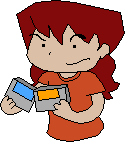
\includegraphics[height=3cm]{images/5-3-games.png}
            \end{wrapfigure}
        
            Rose wants to buy some game cartridges at a garage sale
            but only brought enough cash for two of the four games they have:
            LM: Legacy of Magic, TC: Temporal Catalyst, CC: Concluding Chronicle, and DT: Dream of Terra

            ~\\
            \tab a. What would $n$ be?
            \tab b. What would $r$ be? \\
            \tab c. What is the result of $P(n, r)$?
        \end{question}

    \begin{intro}{Subsets:}
        A \textbf{subset} is a permutation, except that we \textit{do not}
        care about order. So, if we have (2, 3) and (3, 2) as different
        permutations, as two subsets, \{2, 3\} and \{3, 2\} are considered
        the same.
    \end{intro}

        % - QUESTION --------------------------------------------------%
        \begin{question}{4}{15\%}
            
            Going back to Question 3, answer the following questions:

            \begin{enumerate}
                \item[a.] List all the choices that are equivalent to each
                other (example, choosing ``Legacy of Magic" and ``Temporal Catalyst",
                vs. choosing ``Temporal Catalyst" and ``Legacy of Magic".
                
                \item[b.] How many equivalent choices are there?

                \item[c.] So if Rose still selects two games from the four
                possible ones, but the order she selects the games doesn't matter,
                how many different outcomes are there?

            \end{enumerate}
            
        \end{question}


    \newpage
    %------------------------------------------------------------------%
    \section*{3. Equivalence Relations}
    
        % - QUESTION --------------------------------------------------%
        \begin{intro}{Equivalence Relations \& Classes:}\footnote{From Jim Van Horn's notes}
            ~\\
            An \textbf{Equivalence Relation} \\
            $(X, Y) \in R$ if permutations $X$ and $Y$ use the same objects.
            R is the equivalence relation, ``use the same objects."

            ~\\
            An \textbf{Equivalence Class} is the set of objects (in this
            case, permutations) that are equivalent to one another.
            For example, $(Apple, Orange)$ and $(Orange, Apple)$ $\in R$.
            So, these two permutation smake up an equivalence class.

            \paragraph{Example 1:} Given a set of 7 items,
                \{a, s, d, f, j, k, l\}, if we were to choose
                3 items from this set, how many permutations would there be?
                ~\\~\\
                \begin{answer}
                    $P(n,r) => P(7,3) => \frac{7!}{(7-3)!}
                        = \frac{5 \times 4 \times 3 \times 2 \times 1}{4 \times 3 \times 2 \times 1}
                        = \frac{5040}{24}$ \\
                        $= 210$ total permutations
                \end{answer}

                ~\\
                If we were thinking about it in terms of ``buckets" visually, it would look like this:

                \begin{center}
                    \begin{tabular}{c c c}
                        \fitb[2cm] & \fitb[2cm] & \fitb[2cm]
                        \\
                        7 options & 6 options & 5 options
                    \end{tabular}
                    ~\\~\\
                    $= 7 \times 6 \times 5 = $ \textbf{210}
                \end{center}

                \paragraph{Example 2:} For the permutation, \textbf{asd},
                    what are all the elements of the equivalence relation?
                    ~\\~\\
                    \begin{answer}
                        These are all the subsets using \textbf{asd} that would be equivalent.
                        There are a total of \textbf{6} items in the equivalence class, if we
                        are looking at a permutation of length 3.
                        ~\\
                        \{asd, ads, sad, sda, dsa, das\}
                    \end{answer}

                \paragraph{Example 3:} How many subsets of the \{a, s, d, f, j, k, l\}
                    set have 3 elements?
                    ~\\~\\
                    \begin{answer}
                        For this, we divide the amount of permutations of length 3
                        with the amount of items in an equivalence class of length 3. So:
                        $\frac{210}{6} = 35$.
                    \end{answer}
        \end{intro}

        \begin{question}{5}{25\%}
            Given a set \{2000, 2004, 2008, 2012, 2016\}...

            \begin{enumerate}
                \item[a.] How many permutations of length 3 are there?

                \item[b.] For the length-3 permutation of \textbf{2000, 2004, 2008},
                    list out all the permutations in the equivalence class
                    that are related (i.e., ``permutationA and permutationB would
                    be the same if they were subsets".
                
                \item[c.] How many permutations are there in any given
                    equivalence class of length 3?

                \item[d.] How many subsets of length 3 are there for the set \{2000, 2004, 2008, 2012, 2016\}?

                \item[e.] If $n = 5$, the length of our set, and $r = 3$, the length of
                the permutations, what is the result of the following?
                $$C(n,r) = \frac{n!}{(n-r)! \cdot r!}$$
            \end{enumerate}
        \end{question}

    %------------------------------------------------------------------%
    \section*{4. Combinations}

        \begin{intro}{Combinations}
            In mathematics, a combination is selection of items from a collection,
            such that (unlike permutations) the order of selection does not matter.
            (...) The number of $r$-combinations from a given set of $n$ elements
            is often denoted in elementary combinatorics texts by $C(n,r)$.
            \footnote{From https://en.wikipedia.org/wiki/Combinations}

            For a combination of length $r$ from a set of $n$ elements
            is equal to the binomial coefficient,
            $$(^{n}_{r}) = \frac{n(n-1) ... (n-r+1)}{r(r-1)...1}$$
            which can be simplified to:
            $$C(n,r) = \frac{n!}{(n-r)! \cdot r!}$$

            (Note that the book uses $r$ and Wikipedia uses $k$.)
        \end{intro}

        \newpage
        \begin{question}{6}{25\%}
            There are $4!$ possible ways for four students to be seated around a table.
            But, what if we only care about relative position and not the specific chair.
            That is, who you are seated next to - the students on your left and right.
            Assuming there is Alice, Bob, Chen, and David (Going clockwise around the table starting with Alice).

            \begin{center}
                \begin{tabular}{c c c}
                    & A & \\
                    B & & D \\
                    & C &
                \end{tabular}
            \end{center}

            If they were to each move one seat clockwise the arrangement would be: David, Alice, Bob, and Chen.
            This is equivalent to the original arrangement for the relation of ``same person on my left and right".
            \footnote{From Jim Van Horn's POGIL exercises}

            \begin{enumerate}
                \item[a.] How many possible seating arrangements are there?
                \item[b.] How many times can they move one seat clockwise before they are back to their original positions?
                \item[c.] We know that groups of 4 permutations are equivalent when only the relative position is
                    considered and not the specific seat. So, if the equivalence relation is ``same person on my left and right",
                    how many permutations are in each equivalence class? List them all out.
                \item[d.] How many seating arrangements are possible if we are only concerned about how is on our left and who is on our right?
                \item[e.] Instead of individual students, assume that at each table of 4 people, there are two pairs working together against
                    the other team at their table.
                    For a \underline{single team-pair,} how many pair arrangements could there be? List them out.
            \end{enumerate}
        \end{question}
    
    %------------------------------------------------------------------%
    \section*{5. Wind-down}
    
        \begin{question}{6}{12\%}
            Solve the following.
            \begin{center}
                a.   $P(6, 2)$ \tab[3cm]
                b.   $C(6, 2)$ \tab[3cm]
                c.   $C(6, 4)$ \\
                d.   $P(5, 5)$ \tab[3cm]
                e.   $C(5, 5)$ \tab[3cm]
                f.   $C(7, 0)$
            \end{center}
        \end{question}


    %------------------------------------------------------------------%
    %- WORKSHEET ------------------------------------------------------%
    %------------------------------------------------------------------%
    \newpage
    \begin{center} \section*{Chapter \laChapter In-class Exercise Worksheet} \end{center}

    \iftoggle{answerkey}{
      \begin{answer} \begin{center} ANSWER KEY \end{center} \end{answer}
    }{}

    % \iftoggle{answerkey}{ \begin{answer} asdfasdf \end{answer} }{ { ~\\ \raisebox{0pt}[2cm][0pt]{  } } }
    % \iftoggle{answerkey}{ \begin{answer} TRUE \end{answer} }{}

\begin{answersheetquestion}{1}{Function diagram}{5}
    \begin{center}
        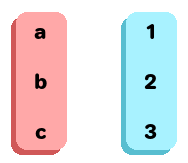
\includegraphics[height=4cm]{images/5-3-question-function.png}
        \iftoggle{answerkey}{ \begin{answer} 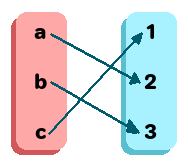
\includegraphics[height=4cm]{images/5-3-question-function-solution.png} \end{answer} }{}
    \end{center}
\end{answersheetquestion}

\hrulefill{}

\begin{answersheetquestion}{2}{Binary relation diagram}{6}
    \begin{center}
        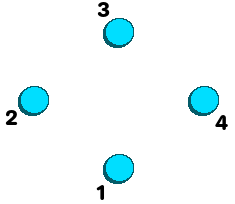
\includegraphics[height=4cm]{images/5-3-question-relation.png}
        \iftoggle{answerkey}{ \begin{answer} 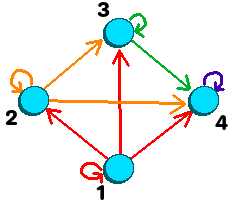
\includegraphics[height=4cm]{images/5-3-question-relation-solution.png} \end{answer} }{}
    \end{center}
\end{answersheetquestion}

\hrulefill{}

\begin{answersheetquestion}{3}{Garage sale games (part 1)}{12}
\begin{enumerate}
    \item[a.] $n$ = \iftoggle{answerkey}{ \begin{answer} 4 \end{answer} }{}
    \item[b.] $r$ = \iftoggle{answerkey}{ \begin{answer} 2 \end{answer} }{}
    \item[c.] $P(n, r)$ = \iftoggle{answerkey}{ \begin{answer} $P(4,2) = \frac{4!}{(4-2)!} = \frac{(4 \cdot 3 \cdot 2 \cdot 1)}{(2 \cdot 1)} = 12$ \end{answer} }{}
\end{enumerate}
\end{answersheetquestion}

\newpage{}

\begin{answersheetquestion}{4}{Garage sale games (part 2)}{15}
\begin{enumerate}
    \item[a.] \iftoggle{answerkey}{ \begin{answer}
        \footnotesize
        (\{ LM, TC \} \{ TC, LM \}), (\{ LM, CC \}, \{ CC, LM \}), (\{ LM, DT \}, \{ DT, LM \}) \\
        (\{ TC, CC \} \{ CC, TC \}), (\{ TC, DT \}, \{ DT, TC \}), \\
        (\{ CC, DT \}, \{ DT, CC \})
        
    \end{answer} }{ { ~\\ \raisebox{0pt}[2cm][0pt]{  } } }
    
    \item[b.]  \iftoggle{answerkey}{ \begin{answer} 6 \end{answer} }{}
    
    \item[c.]  \iftoggle{answerkey}{ \begin{answer} 6 \end{answer} }{}
\end{enumerate}
\end{answersheetquestion}

~\\
\hrulefill{}

\begin{answersheetquestion}{5}{2000 - 2016}{25}
\begin{enumerate}
    \item[a.] \iftoggle{answerkey}{ \begin{answer} $\frac{5!}{(5-3)!} = \frac{120}{2} = 60$ \end{answer} }{}
    
    \item[b.] \iftoggle{answerkey}{ \begin{answer} 2000-2004-2008 \tab 2000-2008-2004 \tab 2004-2000-2008
    \   \\ 2004-2008-2000 \tab 2008-2000-2004 \tab 2008-2004-2000 \end{answer} }{ { ~\\ \raisebox{0pt}[2cm][0pt]{  } } }
    
    \item[c.] \iftoggle{answerkey}{ \begin{answer} 6 \end{answer} }{}
    
    \item[d.] \iftoggle{answerkey}{ \begin{answer} $\frac{60}{6} = 10$ \end{answer} }{}
    
    \item[e.] \iftoggle{answerkey}{ \begin{answer} $C(5,3) = \frac{5!}{(2!)(3!)} = 10$ \end{answer} }{}
\end{enumerate}
\end{answersheetquestion}


\newpage{}

\begin{answersheetquestion}{6}{ABCD Seating}{25}
    \begin{enumerate}
        \item[a.]  \iftoggle{answerkey}{ \begin{answer} $4! = 24$ \end{answer} }{}
        \item[b.]  \iftoggle{answerkey}{ \begin{answer} $4$ \end{answer} }{}
        \item[c.]  \iftoggle{answerkey}{ \begin{answer} 4: ABCD, BCDA, CDAB, DABC
            \end{answer} }{ { ~\\ \raisebox{0pt}[2cm][0pt]{  } } }
        \item[d.] \iftoggle{answerkey}{ \begin{answer} $\frac{24}{4} = 6$ \end{answer} }{}
        \item[e.] \iftoggle{answerkey}{ \begin{answer} 6: AB, AC, AD, BC, BD, CD
            \end{answer} }{ { ~\\ \raisebox{0pt}[2cm][0pt]{  } } }
    \end{enumerate}
\end{answersheetquestion}

~\\
\hrulefill{}

\begin{answersheetquestion}{7}{Wind-down}{12}
    \begin{enumerate}
        \item[a.]   $P(6, 2) =$ \iftoggle{answerkey}{ \begin{answer} $\frac{6!}{4!} = \frac{720}{24} = 30$ \end{answer} }{}
        \item[b.]   $C(6, 2) =$ \iftoggle{answerkey}{ \begin{answer} $\frac{6!}{4! \cdot 2!} = \frac{720}{(24 \cdot 2)} = 15$ \end{answer} }{}
        \item[c.]   $C(6, 4) =$ \iftoggle{answerkey}{ \begin{answer} $\frac{6!}{2! \cdot 4!} = \frac{720}{(2 \cdot 24)} = 15$ \end{answer} }{}
        \item[d.]   $P(5, 5) =$ \iftoggle{answerkey}{ \begin{answer} $\frac{5!}{5!} = \frac{120}{120} = 1$ \end{answer} }{}
        \item[e.]   $C(5, 5) =$ \iftoggle{answerkey}{ \begin{answer} $\frac{5!}{(0! \cdot 5!)} = \frac{5!}{5!} = 1$ \end{answer} }{}
        \item[f.]   $C(7, 0) =$ \iftoggle{answerkey}{ \begin{answer} $\frac{7!}{(7! \cdot 0!)} = \frac{7!}{7!} = 1$ \end{answer} }{}
    \end{enumerate}
\end{answersheetquestion}






    %- Team Info ------------------------------------------------------%

    \newpage
    
    \paragraph{Team:}
    Please write down all people in your team. ~\\

    % table %
    \begin{tabular}{ p{6cm} p{6cm} }
        1. & 2. \\
        3. & 4.
    \end{tabular}
    % table %
    ~\\

    \hrulefill
    \subsection*{Grading}
            
    \begin{center}
        
        \begin{tabular}{ | l | l | l | l | }
            \hline
            \textbf{ Question } & \textbf{ Weight } & \textbf{ 0-4 } & \textbf{ Adjusted score }
            \\ \hline
            
            1 & 5\% & &    \\ \hline
            
            2 & 6\% & &    \\ \hline
            
            3 & 12\% & &    \\ \hline
            
            4 & 15\% & &    \\ \hline
            
            5 & 25\% & &    \\ \hline
            
            6 & 25\% & &    \\ \hline
            
            7 & 12\% & &    \\ \hline
            
            
            
        \end{tabular}
    \end{center}

\end{document}
